\documentclass{standalone}
    \usepackage{tikz}
    \usepackage{pgfplots}
    \usetikzlibrary{calc}
    \usetikzlibrary{patterns}
\mathversion{bold}    
% defining the new dimensions and parameters
\newlength{\hatchspread}
\newlength{\hatchthickness}
\newlength{\hatchshift}
\newcommand{\hatchcolor}{}
% declaring the keys in tikz
\tikzset{hatchspread/.code={\setlength{\hatchspread}{#1}},
         hatchthickness/.code={\setlength{\hatchthickness}{#1}},
         hatchshift/.code={\setlength{\hatchshift}{#1}},% must be >= 0
         hatchcolor/.code={\renewcommand{\hatchcolor}{#1}}}
% setting the default values
\tikzset{hatchspread=3pt,
         hatchthickness=0.4pt,
         hatchshift=0pt,% must be >= 0
         hatchcolor=black}
% declaring the pattern
\pgfdeclarepatternformonly[\hatchspread,\hatchthickness,\hatchshift,\hatchcolor]% variables
   {custom north west lines}% name
   {\pgfqpoint{\dimexpr-2\hatchthickness}{\dimexpr-2\hatchthickness}}% lower left corner
   {\pgfqpoint{\dimexpr\hatchspread+2\hatchthickness}{\dimexpr\hatchspread+2\hatchthickness}}% upper right corner
   {\pgfqpoint{\dimexpr\hatchspread}{\dimexpr\hatchspread}}% tile size
   {% shape description
    \pgfsetlinewidth{\hatchthickness}
    \pgfpathmoveto{\pgfqpoint{0pt}{\dimexpr\hatchspread+\hatchshift}}
    \pgfpathlineto{\pgfqpoint{\dimexpr\hatchspread+0.15pt+\hatchshift}{-0.15pt}}
    \ifdim \hatchshift > 0pt
      \pgfpathmoveto{\pgfqpoint{0pt}{\hatchshift}}
      \pgfpathlineto{\pgfqpoint{\dimexpr0.15pt+\hatchshift}{-0.15pt}}
    \fi
    \pgfsetstrokecolor{\hatchcolor}
%    \pgfsetdash{{1pt}{1pt}}{0pt}% dashing cannot work correctly in all situation this way
    \pgfusepath{stroke}
   }

\begin{document}
\huge
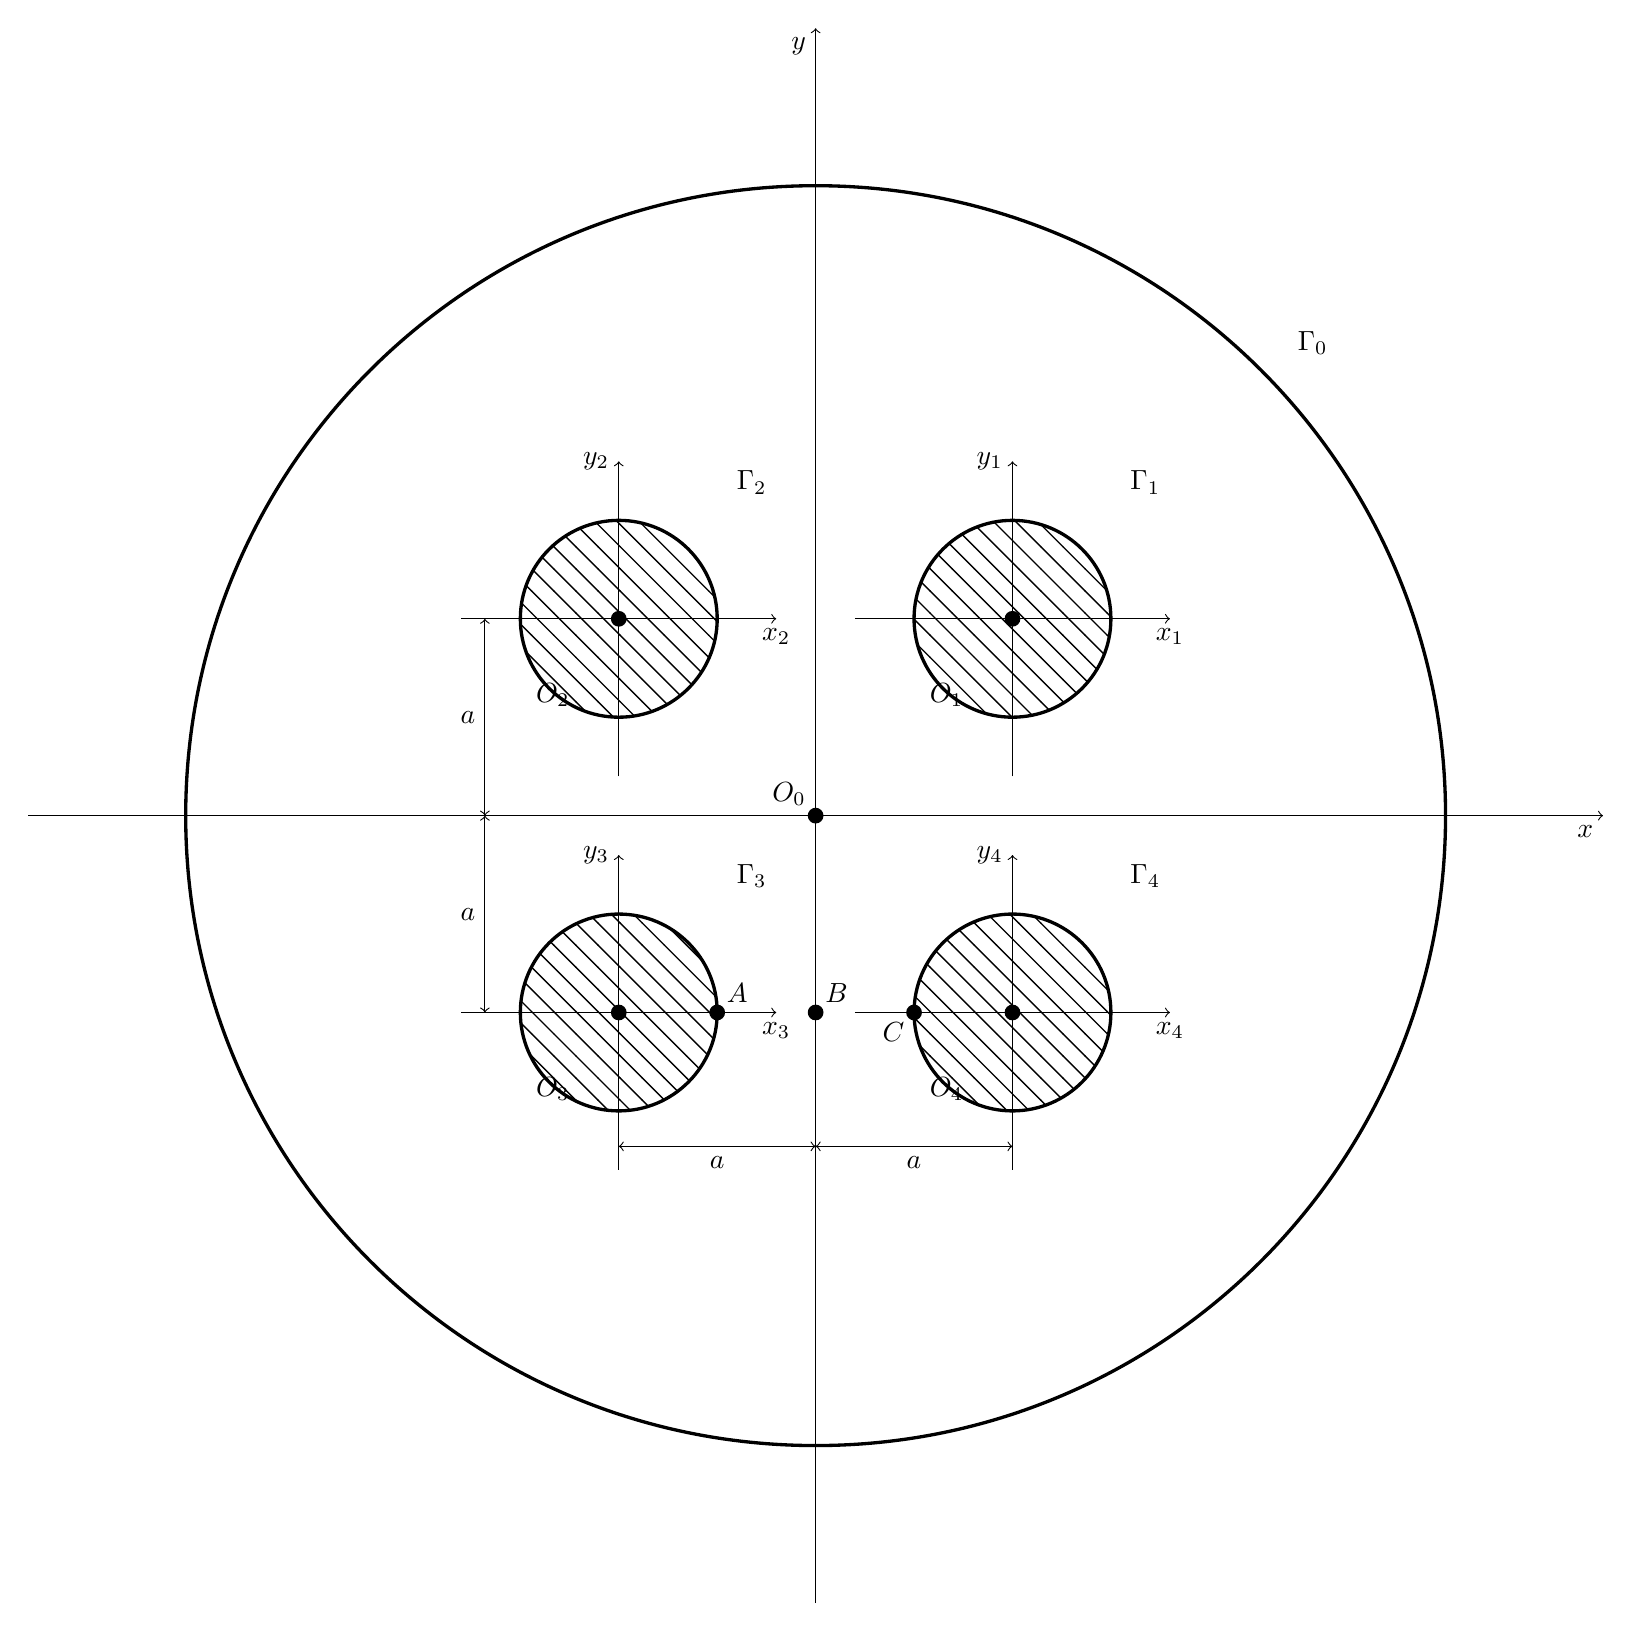
\begin{tikzpicture}[scale=1]
\coordinate (O) at (0,0);
\coordinate (O1) at (2.5,2.5);
\coordinate (O2) at (-2.5,2.5);
\coordinate (O3) at (-2.5,-2.5);
\coordinate (O4) at (2.5,-2.5);
\coordinate (A) at (-1.25,-2.5);
\coordinate (B) at (0,-2.5);
\coordinate (C) at (1.25,-2.5);

\draw[very thick] let \n{radius} = {8.0} in (O) circle (\n{radius});
\draw[->] ($ (-10,0) $) -- ($ (10,0) $) node[below left] {$x$};
\draw[->] ($ (0,-10) $) -- ($ (0,10) $) node[below left] {$y$};

\draw[very thick] (O1) circle (1.25);
\fill[pattern=custom north west lines,hatchspread=8pt,hatchthickness=0.5pt,hatchcolor=black] (O1) circle(1.25);
\node[below left] at (2.0,1.8) {$O_1$};
\node[below left] at (4.5,4.5) {$\Gamma_1$};
\draw[->] (0.5,2.5) -- (4.5,2.5) node[below] {$x_1$};
\draw[->] (2.5,0.5) -- (2.5,4.5) node[left] {$y_1$};

\draw[very thick] (O2) circle (1.25);
\fill[pattern=custom north west lines,hatchspread=8pt,hatchthickness=0.5pt,hatchcolor=black] (O2) circle(1.25);
\node[below left] at (-3.0,1.8) {$O_2$};
\node[below left] at (-0.5,4.5) {$\Gamma_2$};
\draw[->] (-4.5,2.5) -- (-0.5,2.5) node[below] {$x_2$};
\draw[->] (-2.5,0.5) -- (-2.5,4.5) node[left] {$y_2$};

\draw[very thick] (O3) circle (1.25);
\fill[pattern=custom north west lines,hatchspread=8pt,hatchthickness=0.5pt,hatchcolor=black] (O3) circle(1.25);
\node[below left] at (-3.0,-3.2) {$O_3$};
\node[below left] at (-0.5,-0.5) {$\Gamma_3$};
\draw[->] (-4.5,-2.5) -- (-0.5,-2.5) node[below] {$x_3$};
\draw[->] (-2.5,-4.5) -- (-2.5,-0.5) node[left] {$y_3$};

\draw[very thick] (O4) circle (1.25);
\fill[pattern=custom north west lines,hatchspread=8pt,hatchthickness=0.5pt,hatchcolor=black] (O4) circle(1.25);
\node[below left] at (2.0,-3.2) {$O_4$};
\node[below left] at (4.5,-0.5) {$\Gamma_4$};
\draw[->] (0.5,-2.5) -- (4.5,-2.5) node[below] {$x_4$};
\draw[->] (2.5,-4.5) -- (2.5,-0.5) node[left] {$y_4$};

\fill (O) circle(0.1) node[above left] {$O_0$};
\fill (O1) circle(0.1);
\fill (O2) circle(0.1);
\fill (O3) circle(0.1);
\fill (O4) circle(0.1);
\fill (A) circle(0.1) node[above right] {$A$};
\fill (B) circle(0.1) node[above right] {$B$};
\fill (C) circle(0.1) node[below left] {$C$};

\draw[<->] (-4.2,-2.5) -- (-4.2,0);
\node[left] at (-4.2,-1.25) {$a$};
\draw[<->] (-4.2,2.5) -- (-4.2,0);
\node[left] at (-4.2,1.25) {$a$};

\draw[<->] (-2.5,-4.2) -- (0,-4.2);
\draw[<->] (2.5,-4.2) -- (0,-4.2);
\node[below] at (-1.25,-4.2) {$a$};
\node[below] at (1.25,-4.2) {$a$};

\node[right] at (6,6) {$\Gamma_0$};

\end{tikzpicture}
\end{document}

%%% Local Variables: 
%%% mode: latex
%%% TeX-master: t
%%% End: 
